\documentclass[]{article}


% Increase text width
\usepackage[left=48pt,right=46pt]{geometry}

% Grahpics Stuff
\usepackage{graphicx}
\usepackage{float}
\graphicspath{ {images/} }

% Bibliography stuff
\usepackage[round]{natbib}
% Adds bibliography to toc
\usepackage[nottoc,numbib]{tocbibind} 

% Makes toc, urls, figure links
\usepackage{hyperref}

% Format hyperlinks nicer than default way
\usepackage{xcolor}
\hypersetup{colorlinks,linkcolor={blue!80!black},citecolor={blue!80!black},urlcolor={blue!80!black}}

% For inserting code blocks
\usepackage{listings}
\lstset{
	showstringspaces=false,
	basicstyle=\ttfamily,
	columns=fullflexible,
	breaklines=true,
	postbreak=\mbox{\space},
}


\usepackage[title]{appendix}

% Title Page
\title{Docker and AWS Container Exercise\\
	Cloud Technology}
\author{Rob Shelly\\
	Applied Computing\\
	20068406}

\begin{document}
\maketitle
\thispagestyle{empty}

\newpage
\pagenumbering{roman}
\tableofcontents

\newpage
\pagenumbering{arabic}
\section{Docker}

\textit{Dockerising} a simple RabbitMQ system consisted of three containers. One for each of the following: 
\begin{itemize}
	\item RabbitMQ;
	\item A program to emulate a service sending messages;
	\item A program to emulate s service receives messages.
\end{itemize}

\subsection{RabbitMQ Container}
The The RabbitMQ container is the simplest to run. It is run with the following command:
\begin{lstlisting}
docker run -d -e RABBITMQ_NODENAME=my-rabbit --name some-rabbit rabbitmq:3-management
\end{lstlisting}
This pulls prebuilt \textit{RabbitMQ} docker image from Docker Hub and runs it in a container. RabbitMQ is the messaging service for the other services to send and receive messages from/to. Therefore the IP address of the this container is needed so the services can communicate with it. The IP address of the container is found with the following command:
\begin{lstlisting}[language=bash]
IP="$(docker inspect -f '{{ .NetworkSettings.IPAddress }}' rabbit)
\end{lstlisting}

\begin{figure}[H]
	\setlength{\belowcaptionskip}{15pt plus 3pt minus 2pt}
	\caption{RabbitMQ with Two Hello Messages Queued}
	\centering
	%\includegraphics[width=\textwidth,height=\textheight,keepaspectratio]{diagram}
	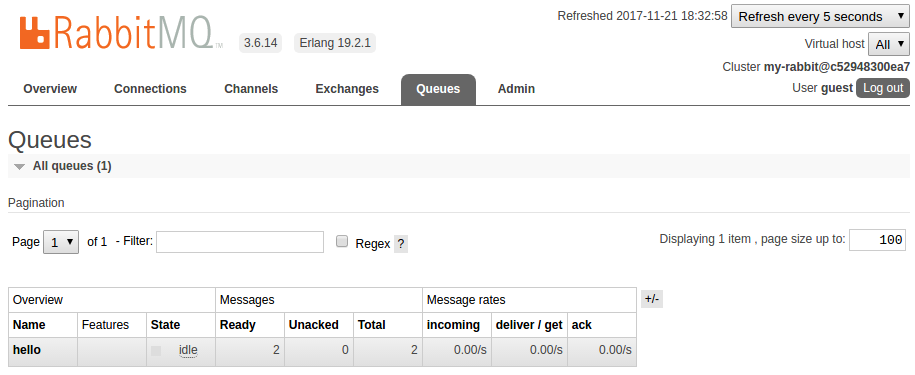
\includegraphics[width=\textwidth,keepaspectratio]{rabbit}
	\label{fig:rabbit}
\end{figure}

\subsection{Send and Receive Containers}
In order to \textit{dockerise} the messaging system images need to be built for the \textit{send} and \textit{receive} programs. In order to do this a Dockerfile is needed (Dockerfiles shown in appendices \ref{send-dockerfile} and \ref{receive-dockerfile}).
Dockerfiles contain commands and instructions for building an image. These include:
\begin{itemize}
	\item \textbf{Base Image:} A base image to use for the build e.g a Ubuntu image;
	\item \textbf{Instructions:} ~Steps necessary to configure the image such as a commands to install required software;
	\item \textbf{Arguments}: Arguments which may be needed for the instructions.
\end{itemize}
For the \textit{send} and \textit{receive} images, the Dockerfiles detail a base Python image, installs the required Pika software and adds the necessary python scripts to send or receive messages(scripts shown in appendices \ref{send-script} and \ref{receive-script}).

The IP address of the RabbitMQ container is also added as a build argument. This allows the scripts to communicate with the RabbitMQ container. In this case it means that the IP address for the messaging service is baked into the image. This may not be desirable as it does not as it does not allow flexibility such as scaling (adding more RabbitMQ containers if necessary). It will be shown later that service discovery can be used for this.

With the Dockerfiles created, the images are built using the following commands:
\begin{lstlisting}[language=bash]
docker build --build-arg rabbitmq_ip=$IP -t send:1 .
docker build --build-arg rabbitmq_ip=$IP -t receive:1 .
\end{lstlisting}

With the images built they are run as follows:
\begin{lstlisting}[language=bash]
docker run -ti send:1 /bin/bash
\end{lstlisting}
This runs the container and opens a terminal to it at which point the send program can be run:
\begin{lstlisting}[language=bash]
chmod +x /code/send.py
/code/send.py
\end{lstlisting}
Similarly for the \textit{receive} program:
\begin{lstlisting}[language=bash]
docker run -ti receive:1 /bin/bash
\end{lstlisting}
This runs the container and opens a terminal to it at which point the send program can be run:
\begin{lstlisting}[language=bash]
chmod +x /code/receive.py
/code/receive.py
\end{lstlisting}

Three containers are now running and messages can be passed as desired by running \textit{send.py} and \textit{receive.py}.

\begin{figure}[H]
	\setlength{\belowcaptionskip}{15pt plus 3pt minus 2pt}
	\caption{Containers Showing Message Passing}
	\centering
	%\includegraphics[width=\textwidth,height=\textheight,keepaspectratio]{diagram}
	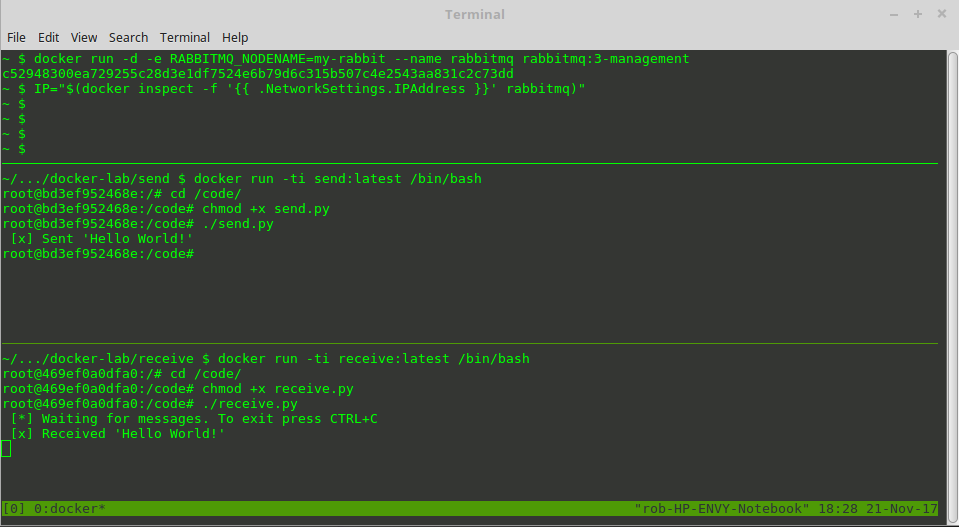
\includegraphics[width=\textwidth,keepaspectratio]{send-receive}
	\label{fig:rabbit}
\end{figure}
\section{AWS EC2 Container Service}
Deploying an app to EC2 Container service consisted of deploying the following service an infrastructure:
\begin{itemize}
	\item ECS Cluster
	\item ECS Optimized EC2 Instance
	\item Task Definition
	\item Application Load Balancer \& Target Group
	\item Service
	\item Application Autoscaling
	\item Scaling Policies \& Cloudwatch Alarms
\end{itemize}
The topology is shown below in \autoref{fig:topology}

\begin{figure}[H]
	\setlength{\belowcaptionskip}{15pt plus 3pt minus 2pt}
	\caption{Topology}
	\centering
	%\includegraphics[width=\textwidth,height=\textheight,keepaspectratio]{diagram}
	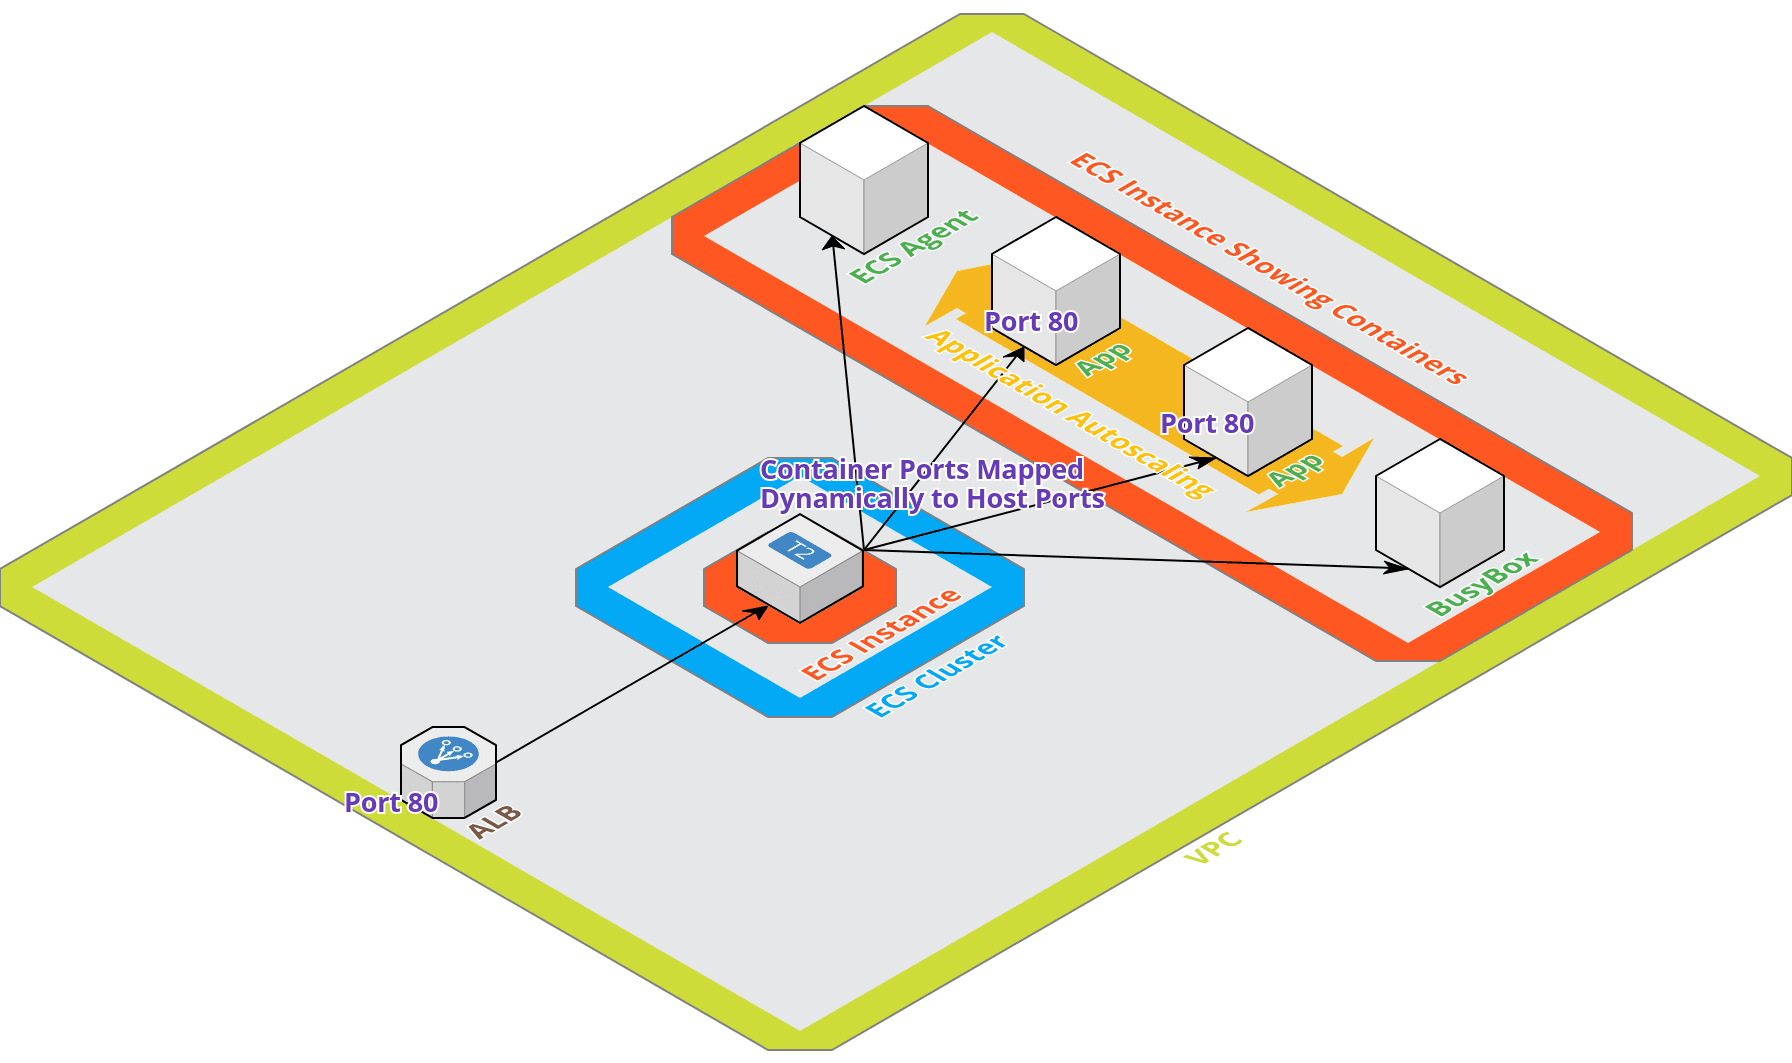
\includegraphics[width=\textwidth,keepaspectratio]{ecs-topology}
	\label{fig:topology}
\end{figure}

\subsection{Setting up the ECS}
The first step was to create an ECS cluster and an instance:
\begin{lstlisting}[language=bash]
aws ecs create-cluster --cluster-name $CLUSTER_NAME
aws ec2 run-instances --image-id $AMI_ID --count 1 --instance-type t2.micro --key-name $KEY_NAME --security-groups $HTTPSSH_SEC_GROUP $VPC_SEC_GROUP --iam-instance-profile Name=$ECS_INSTANCE_ROLE --user-data file://files/user-data.txt --tag-specifications 'ResourceType=instance,Tags=[{Key=Name,Value='$INSTANCE_NAME'}]'
\end{lstlisting}
There are some important parameters to notice here. \textbf{Image ID} is used to specify that an image optimised for ECS is used for the instance. This means that an ECS container agent will be installed and run on the image. The agent allows the instance to connect to a cluster.

The \textbf{VPC Security Group} is used to allow traffic to the instance from it's own VPC. This will be of importance when the application load balancer is added.

\textbf{User Data} is used to specify which cluster to add the instance to. The cluster is a group of ECS instances. Although only one instance will be used in this topology, the cluster allows for application load balancer to occur over many containers over many instances. User data is shown is appendix \ref{user-data}).


Next a task definition is created.
\begin{lstlisting}[language=bash]
aws ecs register-task-definition --cli-input-json file://simple-app-task-def.json
\end{lstlisting}

A task definition contains instructions for running a container on the instance.  It specifies the image to run and where to pull the image from (i.e ECS registry or an external registry such Docker Hub. The task definitions used specifies the simple php-app contained on Docker Hub. It also details port numbers to be used. For this implementation, in which an application load balancer and multiple container apps will be used, the task definition specifies that the container should use port 80. It also specifies that the host port used should be 0. This will dynamically map a random port number of the host to port 80 the container. This is necessary because multiple container apps will run on the instance so they cannot all be accessed via port 80. The task definition can be seen in appendix \ref{task-definition}.
Also detailed in the task definition is the resources allocated to each container. In order to allow all the necessary containers to run on the \textit{t2.micro} used in this topology, tall containers were allocated 100MiB, including the \textit{BusyBox} container.

\subsection{Load Balancing}
Load balancing is achieved using an Application load balancer (ALB). The an ALB has the ability to balance traffic across multiple apps running in multiple containers on one or more instances.
\begin{lstlisting}[language=bash]
aws elbv2 create-load-balancer --type application --name $LB_NAME --security-groups $HTTPSSH_SEC_GROUP_ID $VPC_SEC_GROUP_ID --subnets $SUBNET_A_ID $SUBNET_B_ID $SUBNET_C_ID
\end{lstlisting}
A target group is also created and the instance registered one it. This tell the ALB where to route traffic.
\begin{lstlisting}[language=bash]
aws elbv2 create-target-group --name $TG_NAME --protocol HTTP --port 80 --vpc-id $VPC_ID --target-type instance --health-check-protocol HTTP --health-check-path "/index.php"
aws elbv2 register-targets --target-group-arn $TG_ARN --targets Id=$INSTANCE_ID
\end{lstlisting}
The target group is the instance on which the containers are running. It registers the app containers as targets for the ALB via the host port numbers which have been dynamically allocated according to the task definition (as mentioned above). It also monitors the health of the containers health check.

An listener is added to the ALB and configured to use the target group. This listens on the configured port (80 in this case) of the ALB and routes traffic to the correct ports for the app containers (registered through the instance to the target group).
\begin{lstlisting}[language=bash]
aws elbv2 create-listener --load-balancer-arn $LB_ARN --protocol HTTP --port 80 --default-actions Type=forward,TargetGroupArn=$TG_ARN
\end{lstlisting}
The ALB has been configured with a security that allows inbound HTTP traffic. This allows web browser to view the app using the ALBs address. However, as described, the ALB routes traffic to the app containers on the dynamically allocated port numbers. It can't direct traffic to numerous containers all using port 80. Therefore, the same security group won't allow traffic to the instance, and therefore will prevent the apps displaying when visiting the ALBs address. This is the reason the VPC security group was used when creating the instance above. The instance will allow traffic from inside it's own VPC, which includes the ALB.

\subsection{Service}
The service is used to scale the web app. If only a single container running the web app was needed a service would not be required (or the ALB) and the task definition created above could be run (using host port 80). However a service can be used to run multiple task definitions behind the ALB according to an application autoscaling policy. The ECS instance is registered and a scalable target for service.
\begin{lstlisting}[language=bash]
aws ecs create-service --cluster $CLUSTER_NAME --service-name $SERVICE_NAME --task-definition $TASK_DEF:$REVISION --load-balancers targetGroupArn=$TG_ARN,containerName=$CONTAINER_NAME,containerPort=80 --desired-count 2 --role $ECS_SERVICE_ROLE
aws application-autoscaling register-scalable-target --service-namespace ecs --resource-id service/$CLUSTER_NAME/$SERVICE_NAME --scalable-dimension ecs:service:DesiredCount --min-capacity 1 --max-capacity 3 --role-arn $APP_AUTOSCALING_ROLE_ARN
\end{lstlisting}
Once the service is created with a desired number of task set to a number greater than zero and application autoscaling is configure, the service will automatically start the desired number of instance. I.e. Autoscaling will not occur because there are no policies configured than simple scaling to the desired number of tasks. The app can now be view through the ALB ash shown in \autoref{fig:app}

\begin{figure}[H]
	\setlength{\belowcaptionskip}{15pt plus 3pt minus 2pt}
	\caption{Simple Web App Running Behind Application Load Balancer}
	\centering
	%\includegraphics[width=\textwidth,height=\textheight,keepaspectratio]{diagram}
	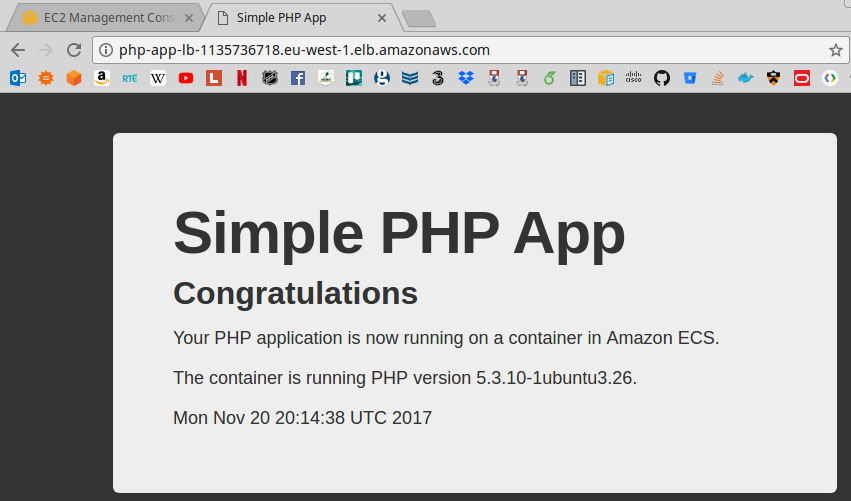
\includegraphics[width=\textwidth,keepaspectratio]{php-app-working}
	\label{fig:app}
\end{figure}


\subsection{Application Autoscaling}
Finally the scaling policies and their corresponding cloudwatch alarms are created for the application autoscaling.
This consists of three main components, the scaling policies, scaling actions and cloud watch alarms.
First the scaling policies are defined. This defines the scalable resource, i.e. the desired count of the service and the type of scaling to implement (Step scaling in this case).
\begin{lstlisting}[language=bash]
aws application-autoscaling put-scaling-policy --policy-name $SCALE_OUT_POLICY_NAME  --service-namespace ecs --resource-id service/$CLUSTER_NAME/$SERVICE_NAME --scalable-dimension ecs:service:DesiredCount --policy-type StepScaling --step-scaling-policy-configuration="AdjustmentType=ChangeInCapacity,StepAdjustments=[{ScalingAdjustment=0,MetricIntervalLowerBound=0}],MetricAggregationType=Average,Cooldown=60"
aws application-autoscaling put-scaling-policy --policy-name $SCALE_IN_POLICY_NAME  --service-namespace ecs --resource-id service/$CLUSTER_NAME/$SERVICE_NAME --scalable-dimension ecs:service:DesiredCount --policy-type StepScaling --step-scaling-policy-configuration="AdjustmentType=ChangeInCapacity,StepAdjustments=[{ScalingAdjustment=0,MetricIntervalLowerBound=0}],MetricAggregationType=Average,Cooldown=60"
\end{lstlisting}
Then the cloudwatch alarms are created. These monitor some resource, CPU utilisation in this case, and trigger actions when certain limits are met. 
\begin{lstlisting}[language=bash]
aws cloudwatch put-metric-alarm --alarm-name $SCALE_OUT_ALARM_NAME --metric-name CPUUtilization --namespace AWS/ECS --statistic Average --dimensions "Name=ClusterName,Value=php-app Name=ServiceName,Value=php-app-service" --period 60 --evaluation-periods 60 --comparison-operator GreaterThanOrEqualToThreshold --threshold 75 --unit Percent --actions-enabled --alarm-actions $SCALE_OUT_POLICY_ARN
aws cloudwatch put-metric-alarm --alarm-name $SCALE_IN_ALARM_NAME --metric-name CPUUtilization --namespace AWS/ECS --statistic Average --dimensions "Name=ClusterName,Value=php-app Name=ServiceName,Value=php-app-service" --period 60 --evaluation-periods 60 --comparison-operator LessThanOrEqualToThreshold --threshold 25 --unit Percent --actions-enabled --alarm-actions $SCALE_IN_POLICY_ARN
\end{lstlisting}
However, while completing this exercise it was noted that configuring a scalable action for a namespace of AWS ECS was impossible using the CLI. Therefore this step was carried out though the AWS console.

\section{Service Discovery}
In the first section of this paper demonstrated how to containerised services in a messaging system. However, in order for the sending and receiving containers to communicate with the RabbitMQ container they need to have the IP address of the RabbitMQ container hard coded. This does not provide great flexibility. For example, autoscaling the RabbitMQ service cannot be achieved with this setup as other containers won't know the IP address of the new containers created through scaling. This creates the need for service discovery. Service discovery manages the communication of distributed service in a micro-service architecture. The service discovery tool used in this exercise is Consul.

\subsection{Setting up the System}
The system for this exercise consisted of three services running on a single ECS instance: A weather service for reporting weather details, a stock-price service for reporting stock prices and a portal which acts as a fronted for the aforementioned services. Therefore, the portal needs a way of communication with the weather and stock-price containers. Source code for these services was obtained from Github.

To create the system an ECS cluster is first created. The remaining architecture was created using a CloudFormation template obtained with the services course code and a small number of parameters, including a VPC, a subnet and Amazon DNS IP.

The Amazon DNS is a DNS server created by default in a VPC to allows instance within the VPC to talk to the VPC's Internet gateway. The IP address server can be accessed by subnest of the VPC at the network address of the subnet plus two i.e. if the subnet address is 172.31.0.0/16 then the Amazon DNS IP is 172.31.0.2. Therefore, when inserting the parameters for the CloudFormation stack it is important to ensure the subnet enter is contained within the VPC entered and that the DNS IP is the address of for that subnet.

Once the stack created and 2 EC2 instances are created. One contains the Consul Server and the other is an ECS instance which has been added to the cluster created earlier. The ECS instance is where the service will run in containers. On creation it is running a containing with a Consul agent. It is the agent that provides the service discovery mechanism to the other containers, e.g. it will allows the portal to discover and hence make requests to the weather and stock-price services.

The services were built by logging onto the Consul server instance, cloning the source code and then building images using Dockerfiles. The images where then pushed to Docker Hub.

Finally, a task definition and a service to run each image once the ECS instance was created, similar to the ECS section of this report. However, this time the ALB and Application Autoscaling policies were omitted, instead just selecting a desired number of tasks as one, for each service.

\begin{figure}[H]
	\setlength{\belowcaptionskip}{15pt plus 3pt minus 2pt}
	\caption{Portal}
	\centering
	%\includegraphics[width=\textwidth,height=\textheight,keepaspectratio]{diagram}
	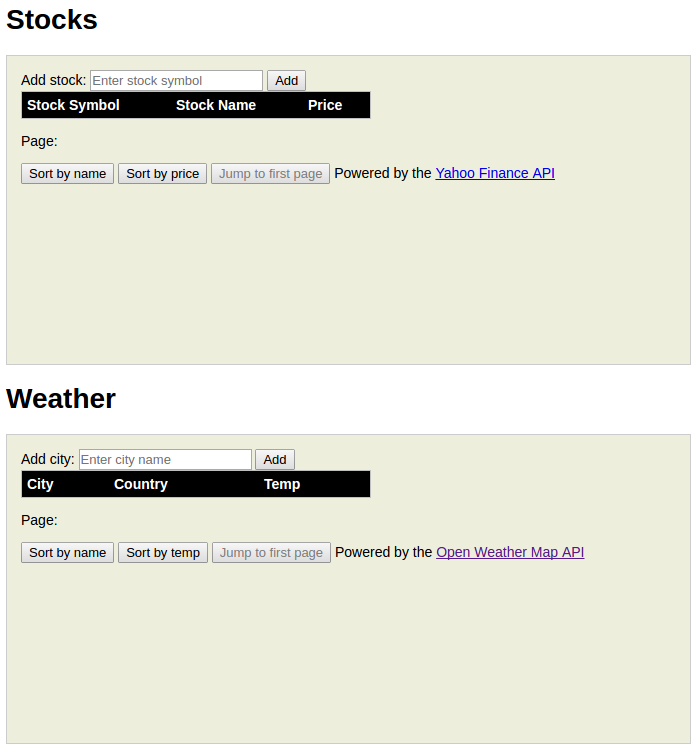
\includegraphics[width=\textwidth,keepaspectratio]{stocks-and-weather}
	\label{fig:rabbit}
\end{figure}
\section{Conclusion}
Section one of this paper demonstrated how micro-services can be deployed in a containerised environment using Docker. This was achieved by deploying a messaging system, RabbitMQ, and two services for sending and receiving messages. Containerising services has many benefits including improving scalability.

In the second section of paper the ability to scale and load balance across containers was explored. If this was attempted using the same methods utilised in section one however it would have been much more difficult. This paper used a simple web app to demonstrate scaling. This web app is accessible on port 80. However, when containerised on a single machine, scaling becomes more difficult as scaling the app to add more containers on the machine causes a problem with ports. I.e. two containers cannot both listen on the same port number if they are running on the same machine. This problem would have manifested in section one if the RabbitMQ service was scaled or replicated for redundancy. Two RabbitMQ server containers could not have listened on the same port number!

This problem was overcome by using AWS services to deploy the web app. The app containers were deployed to an ECS instance running and ECS cluster with autoscaling service configured. An application load balancer was then used to balance traffic between the apps running in containers. The apps listen on port 80 of their respective containers  but each container was mapped to an arbitrary port of the host (achieved though simple settings in the task definition). The target group for the ALB takes care of this mapping. It registers the containers on the ECS instance and allows the ALB to route traffic to the host ports for the containers.

The use of these AWS service means that port mapping does not have to be manually configured for the ports as autoscaling occurs. If this system was configured trough the use of Docker alone, as in section one, manual configuration would be necessary.

The third section of paper addressed another issue raised by the deployment of the messaging system. As demonstrated, this required the IP address of the RabbitMQ servers container to be hard-coded into the service that send and receive messages. This is not a satisfactory implementation as it does not allow easy autoscaling. IP addresses hard-coded into the other service would need to be updated every time a RabbitMQ container is created or destroyed.

This issue was overcome through the use of Consul. Consul is a service discovery tool that allows services to communicate by detecting new services/containers as they appear. Services can query the consul server or a consul agent (which runs on services maintaining health checks) when they need to discover other services.

As shown, the use of various tools or service can manage the issues that arise from a simple micro service architecture such as the messaging system demonstrated in section one. This paper demonstrated how the use of the service discovery tool Consul along with the container management service ECS allows for easier autoscaling and load balancing.

\begin{appendices}
\section{Dockerfile for Send Container} \label{send-dockerfile}
\begin{lstlisting}
FROM python:2

RUN pip install pika

ADD send.py /code/send.py
ARG rabbitmq_ip
RUN sed -i s/rabbitmq_ip/$rabbitmq_ip/g /code/send.py
\end{lstlisting}

\section{Python Script to Send Messages} \label{send-script}
\begin{lstlisting}[language=python]
#!/usr/bin/env python
import pika


# Need ip address of RabbitMQ container
connection = pika.BlockingConnection(pika.ConnectionParameters('rabbitmq_ip'))
channel = connection.channel()


channel.queue_declare(queue='hello')


channel.basic_publish(exchange='',
routing_key='hello',
body='Hello World!')
print(" [x] Sent 'Hello World!'")

connection.close()
\end{lstlisting}
\section{Dockerfile for Receive Container} \label{receive-dockerfile}
\begin{lstlisting}
FROM python:2

RUN pip install pika

ADD receive.py /code/receive.py
ARG rabbitmq_ip
RUN sed -i s/rabbitmq_ip/$rabbitmq_ip/g /code/receive.py
\end{lstlisting}

\section{Python Script to Receive Messages} \label{receive-script}
\begin{lstlisting}[language=python]
#!/usr/bin/env python
import pika


# Need ip address of RabbitMQ container
connection = pika.BlockingConnection(pika.ConnectionParameters('rabbitmq_ip'))
channel = connection.channel()


channel.queue_declare(queue='hello')

def callback(ch, method, properties, body):
print(" [x] Received %r" % body)


channel.basic_consume(callback,
queue='hello',
no_ack=True)

print(' [*] Waiting for messages. To exit press CTRL+C')
channel.start_consuming()
\end{lstlisting}
\section{User Data} \label{user-data}
\begin{lstlisting}[language=bash]
#!/bin/bash	
echo ECS_CLUSTER=RFClusterdemo >> /etc/ecs/ecs.config	
\end{lstlisting}

\section{Task Defninition} \label{task-definition}
\begin{lstlisting}[language=bash]
{
	"family": "php-app",
		"volumes": [
			{
				"name": "my-vol",
				"host": {}
			}
		],
	"containerDefinitions": [
		{
			"environment": [],
			"name": "simple-app",
			"image": "rshelly/amazon-ecs-sample",
			"cpu": 10,
			"memory": 100,
			"portMappings": [
				{
					"containerPort": 80,
					"hostPort": 0
				}
			],
			"mountPoints": [
				{
					"sourceVolume": "my-vol",
					"containerPath": "/var/www/my-vol"
				}
			],
			"entryPoint": [
				"/usr/sbin/apache2",
				"-D",
				"FOREGROUND"
			],
			"essential": true
		},
		{
			"name": "busybox",
			"image": "busybox",
			"cpu": 10,
			"memory": 100,
			"volumesFrom": [
			{
				"sourceContainer": "simple-app"
			}
			],
			"entryPoint": [
				"sh",
				"-c"
			],
			"command": [
				"/bin/sh -c \"while true; do /bin/date > /var/www/my-vol/date; sleep 1; done\""
			],
			"essential": false
		}
	]
}

\end{lstlisting}

\end{appendices}

\end{document}


